% !TeX spellcheck = ru_RU
% !TeX encoding = UTF-8
\subsection{Передача сигнала по беспроводному каналу в комплексной форме}
Сигналы  квадратурной  амплитудной  модуляции(КАМ) (quadrature amplitude modulation, QAM) имеют вид  $s_{i}(t)=s_{i1}(t)\varphi_{1}(t)+s_{i2}(t)\varphi_{2}(t)$, где $\varphi_{1},\varphi_{2}$--- это две  ортонормированные  функции,  заданные  на  интервале $[0,T]$  и определяющие форму сигнала, $i=0,1,..,q-1$. Величины $ s_{i1},s_{i2}$   для  сигналов  КАМ  принимают дискретные  значения  равномерно  расположенные  в  некотором  конечном интервале.  Они  могут  рассматриваться  как  амплитудные  множители  при функциях $\varphi_{1}$ и $\varphi_{2}$, поэтому сигнал КАМ представляет собой сумму двух ортогональных АМ сигналов $s_{i1}(t)\varphi_{1}(t)$ и $s_{i2}(t)\varphi_{2}(t)$.
Как обычно будем считать, что $q=2^{m} $ , где  $m$--- целое; число $m$ может рассматриваться  как  число  бит  переносимых  сигналом(при отсутствии кодирования).
\begin{equation}
s_{i1}=A(1-\dfrac{2i_{1}}{\sqrt{q}-1}),s_{i2}=A(1-\dfrac{2i_{2}}{\sqrt{q}-1}), 
\end{equation} 
где $A$--- максимальное абсолютное значение величин $s_{i1}$ и $s_{i2}$. Очевидно, что значения  величин $ s_{i1}$ и $s_{i2}$ расположены  с  равномерным  шагом  в интервале $[-A,A]$.Сигнальное множество КАМ показано на рис ~\ref{fig:mal1}

\begin{figure}[H]
	\centering
	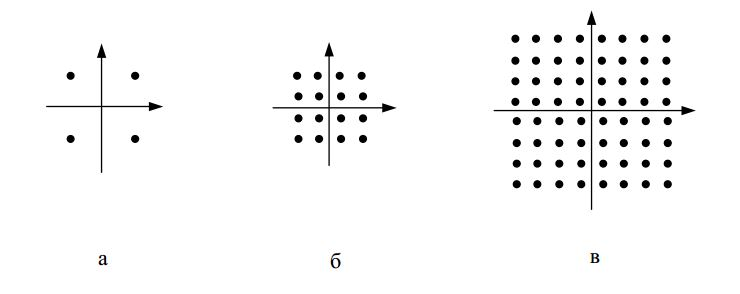
\includegraphics[width=0.5\textwidth]{img/mal1}
	\caption{Сигнальное множество КАМ а)$q=4$ б)$q=16$ в)$q=64$ }
	\label{fig:mal1}
\end{figure}

Напишим моделирующую программу КАМ для передачи $q=4$ сигналов. При моделировании базисные функции будут выглядить как на рисунке ~\ref{fig:mal2} и задаются выражениями вида 

\begin{equation}
\varphi_{1}(t)=\sqrt{\dfrac{2}{T}}\cos2\pi f_{0}t,
\varphi_{2}(t)=\sqrt{\dfrac{2}{T}}\sin2\pi f_{0}t.
\end{equation} 

\begin{figure}[H]
	\centering
	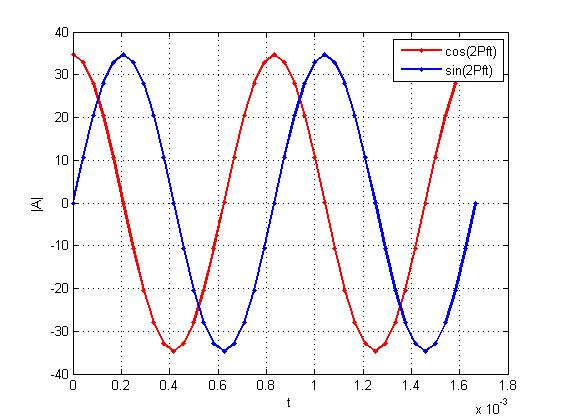
\includegraphics[width=0.5\textwidth]{img/mal2}
	\caption{Вид базисных функций сигнала КАМ}
	\label{fig:mal2}
\end{figure}
  
Используя ранее написаный выражения можно получить представление о внешнем виде сигналов во временной области.
  \begin{figure}[H]
  	\centering
  	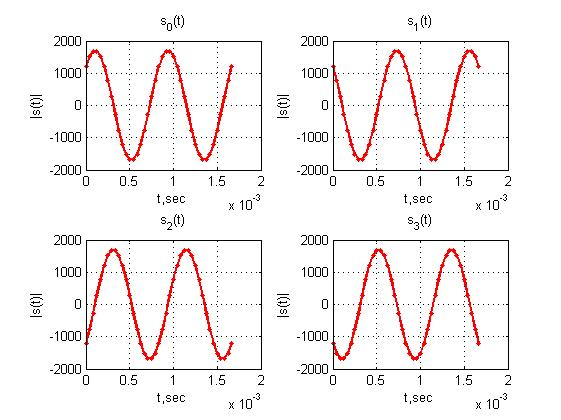
\includegraphics[width=0.5\textwidth]{img/mal3}
  	\caption{Внешний вид всех сигналов сигнального множества}
  	\label{fig:mal3}
  \end{figure}
Спектр сигнала вычисляется согласно формуле прямого преобразования Фурье
\begin{equation}
S_{i}(f)=\int s_{i}(t)e^{-j2\pi f_{t}}dt,
\end{equation}
где $i$---номер преобразуемого сигнала $i=0,1,..,q-1$. Для сигналов квадратурной амплитудной модуляции спектр вычисляется следующим образом:
\begin{equation}
S_{i}(f)=S_{ci}(f)+S_{si}(f),
\end{equation}
где $ S_{ci}(f),S_{si}(f) $--- косинусная и синусная части спектра, определяемые выражениями:
\begin{equation}
S_{ci}(f)=(s_{i1}\frac{T}{2})(sinc((f-f_{0})T)+sinc((f-f_{0})T)),
\end{equation}

\begin{equation}
S_{si}(f)=(s_{i2}\frac{T}{2j})(sinc((f-f_{0})T)+sinc((f-f_{0})T)).
\end{equation}
Ниже представлены графики спектров всех сигналов сигнального множества

\begin{figure}[H]
 	\centering
 	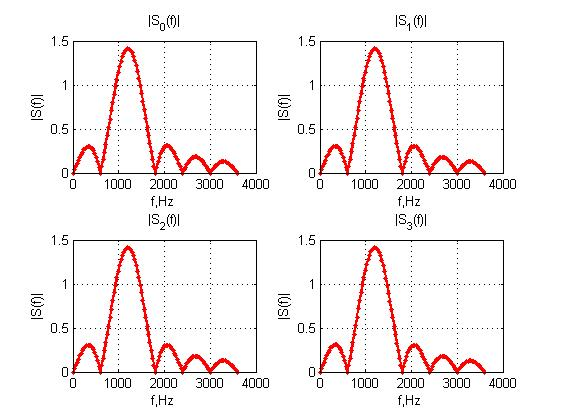
\includegraphics[width=0.5\textwidth]{img/mal4}
 	\caption{Внешний вид спектров всех сигналов сигнального множества}
 	\label{fig:mal4}
\end{figure}
Спектр последовательности сигналов вычисляется согласно выражению:
\begin{equation}
S_{i}(f)=\sum S_{i_{l}}(f)e^{-j2\pi flT},
\end{equation}
где N --- длина последовательности; $i=(i_{0},i_{1},...,i_{N-1})$--- индексы сигналов, входящих в последовательность; $(0\leq l\leq N-1)$ --- номер сигнала в последовательности; 
Ниже представлены графики спектра последовательности сигналов для случайной последовательности ~\ref{fig:mal5}.
\begin{figure}[H]
	\centering
	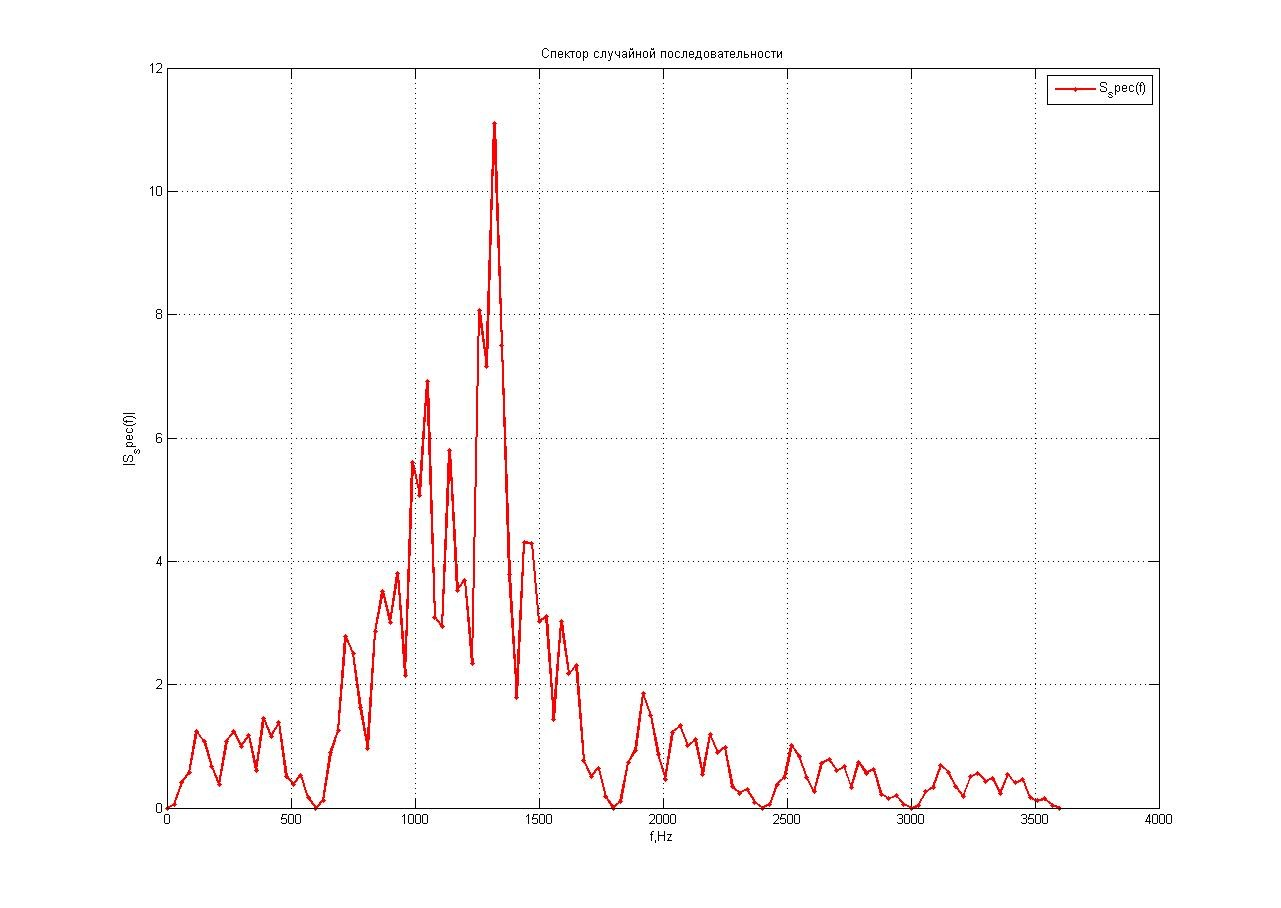
\includegraphics[width=0.5\textwidth]{img/mal5}
	\caption{Спектр последовательности сигналов.}
	\label{fig:mal5}
\end{figure} 
 
 На приемной стороне сами координаты сигнальных точек можно получить перемножением исходного сигнала   на ортогональные базисные функции $ \varphi_{1}(t)$ и $\varphi_{2}(t)$. Сигнальное множество для квадратурной амплитудной модуляции представлено на рисунке ~\ref{fig:mal6}.
 
 \begin{figure}[H]
 	\centering
 	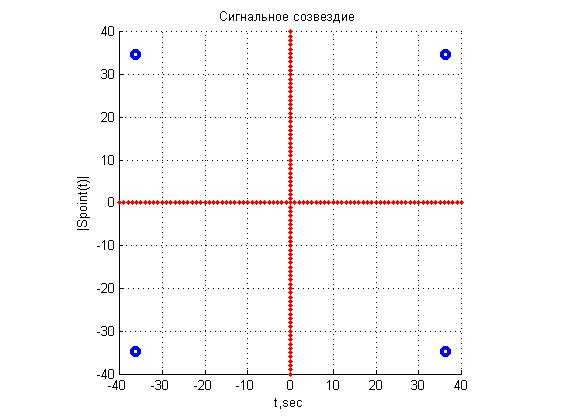
\includegraphics[width=0.5\textwidth]{img/mal6}
 	\caption{Решающие области КАМ для q = 4.}
 	\label{fig:mal6}
 \end{figure} 
\subsection{Исследование оптимального приемника}

В канале с аддитивным белым гауссовским шумом (АБГШ) происходит искажение исходного сигнала согласно выражению  $r(t)=s(t)+n(t)$, где --- передаваемый сигнал, $n(t)$ --- нормально распределенная случайная величина с нулевым математическим ожиданием и нулевой дисперсией,$r(t)$ --- сигнал, полученный непосредственно на выходе канала.
Схематичное представление оптимального приемника представлено на рисунке ~\ref{fig:mal7}.

 \begin{figure}[H]
	\centering
	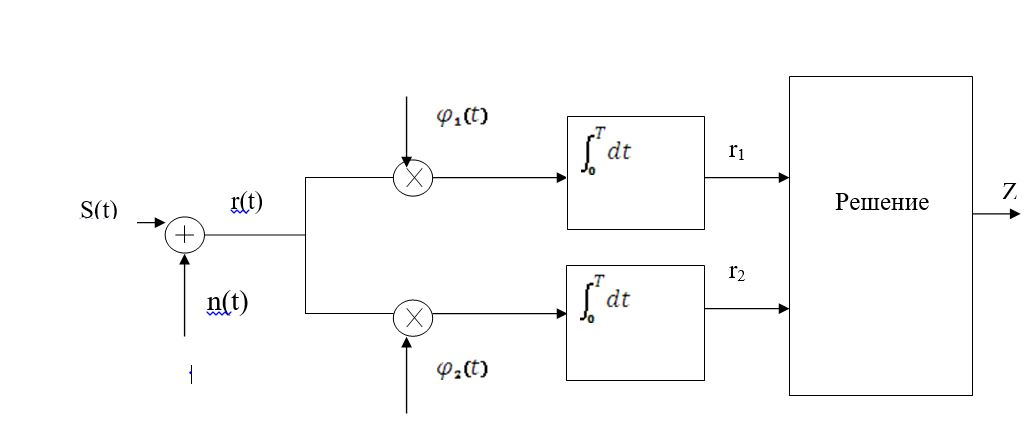
\includegraphics[width=0.5\textwidth]{img/mal7}
	\caption{Схема оптимального приемника.}
	\label{fig:mal7}
\end{figure} 
Наличие шума в канале приводит к  неточному отображению сигнала $s_{i}$  в точку сигнального созвездия $i$, в результате чего вокруг данной точки образуется облако рассеивания. Размер этого облака уменьшается с ростом отношения сигнал-шум.
 \begin{figure}[H]
	\centering
	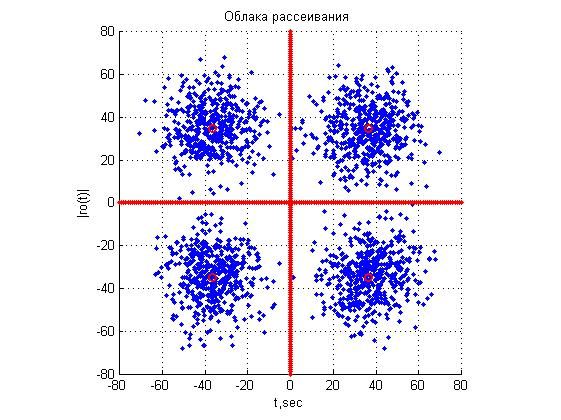
\includegraphics[width=0.5\textwidth]{img/mal8}
	\caption{Облако рассеивания для КАМ=4}
	\label{fig:mal8}
\end{figure} 
При возрастании отношения сигнал шум возрастает вероятность ошибки при декодировании.
Одной из важнейших характеристик приемника является вероятность ошибки. Для сигналов КАМ-4 вероятность ошибки оценивается следующей формулой:

\begin{equation}
P_{e}=1-(1-2Q(\sqrt{\dfrac{6E}{N_{0}(q-1)}}))
\end{equation}
 
где $\dfrac{E}{N_{0}}$--- отношение сигнал-шум в канале; $Q(x)$ --- табличная функция, задается выражением:
\begin{equation}
Q(x)=\dfrac{1}{\sqrt{2\pi}}\int e^{\frac{z_{2}}{2}}dz
\end{equation}
Используя данные выражения можно получить зависимость вероятности ошибки от отношения сигнал-шум.

 \begin{figure}[H]
	\centering
	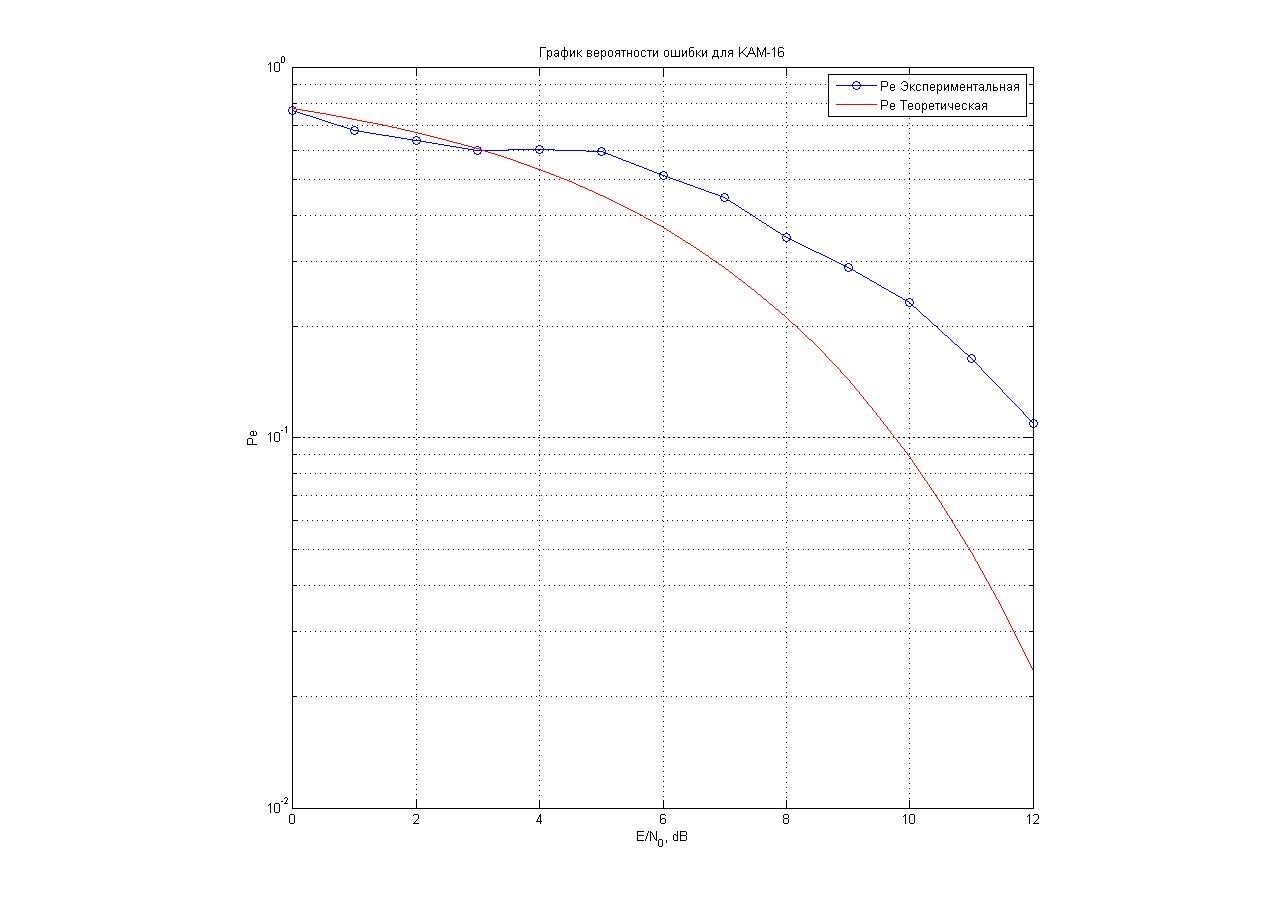
\includegraphics[width=0.5\textwidth]{img/mal9}
	\caption{Теоретическое и практическое значение вероятности ошибки}
	\label{fig:mal9}
\end{figure}
Во время выполнения работы, методом статистического моделирования, была получена оценка вероятности ошибочного приема сигнала с помощью отношения сигнал-шум, что позволило произвести сравнение теоретического и практического значений вероятности ошибки.
Как видно из рисунка ~\ref{fig:mal9} экспериментальное значение вероятности ошибки совпадает с теоретическим.
Их различие объясняется тем , что при проектировании и получении значений вероятности ошибки были округления выходные величины, которые в свою очередь уже дали не точные данные. Также различия произошли при использовании$ Q(x)$ функции, так как ее реализация для программирования тоже имела место округления выходных величин.

Код программы на Matlab [\ref{code:Malahova.code1}]:
\lstinputlisting[language=Matlab, frame=single,
label=code:Malahova.code1, caption=Листинг программы]
{src/tu.m}
%\lstinputlisting[language=Matlab, label=code:code1, captionpos=b, caption=Программа моделирования]{tu/1.m}
Код программы на Matlab [\ref{code:Malahova.code2}]:
\lstinputlisting[language=Matlab, frame=single,
label=code:Malahova.code2, caption=Листинг программы]
{src/Qfun.m}
%\lstinputlisting[language=Matlab, label=code:code1, captionpos=b, caption=Программа моделирования]{Qfun/1.m}

